%%%%%%%%%%%%%%%%%%%%%%%%%%%%%%%%%%%%%%%%%
% Beamer Presentation
% LaTeX Template
% Version 1.0 (10/11/12)
%
% This template has been downloaded from:
% http://www.LaTeXTemplates.com
%
% License:
% CC BY-NC-SA 3.0 (http://creativecommons.org/licenses/by-nc-sa/3.0/)
%
%%%%%%%%%%%%%%%%%%%%%%%%%%%%%%%%%%%%%%%%%

%----------------------------------------------------------------------------------------
%	PACKAGES AND THEMES
%----------------------------------------------------------------------------------------

\documentclass{beamer}

\mode<presentation> {

% The Beamer class comes with a number of default slide themes
% which change the colors and layouts of slides. Below this is a list
% of all the themes, uncomment each in turn to see what they look like.

%\usetheme{default}
%\usetheme{AnnArbor}
%\usetheme{Antibes}
%\usetheme{Bergen}
%\usetheme{Berkeley}
%\usetheme{Berlin}
%\usetheme{Boadilla}
%\usetheme{CambridgeUS}
%\usetheme{Copenhagen}
%\usetheme{Darmstadt}
%\usetheme{Dresden}
%\usetheme{Frankfurt}
%\usetheme{Goettingen}
\usetheme{Hannover}
%\usetheme{Ilmenau}
%\usetheme{JuanLesPins}
%\usetheme{Luebeck} //die schaut gut aus
%\usetheme{Madrid}
%\usetheme{Malmoe}
%\usetheme{Marburg}
%\usetheme{Montpellier}
%\usetheme{PaloAlto}
%\usetheme{Pittsburgh}
%\usetheme{Rochester}
%\usetheme{Singapore}
%\usetheme{Szeged}
%\usetheme{Warsaw}

% As well as themes, the Beamer class has a number of color themes
% for any slide theme. Uncomment each of these in turn to see how it
% changes the colors of your current slide theme.

%\usecolortheme{albatross}
%\usecolortheme{beaver}
%\usecolortheme{beetle}
%\usecolortheme{crane}
%\usecolortheme{dolphin}
%\usecolortheme{dove}
%\usecolortheme{fly}
%\usecolortheme{lily}
%\usecolortheme{orchid}
%\usecolortheme{rose}
%\usecolortheme{seagull}
%\usecolortheme{seahorse}
%\usecolortheme{whale}
%\usecolortheme{wolverine}

%\setbeamertemplate{footline} % To remove the footer line in all slides uncomment this line
%\setbeamertemplate{footline}[page number] % To replace the footer line in all slides with a simple slide count uncomment this line

\setbeamertemplate{navigation symbols}{} % To remove the navigation symbols from the bottom of all slides uncomment this line
}

\usepackage{graphicx} % Allows including images
\usepackage{booktabs} % Allows the use of \toprule, \midrule and \bottomrule in tables

\usepackage{listings}
\usepackage{xcolor}
\lstset { %
    language=C++,
    %backgroundcolor=\color{black!5}, % set backgroundcolor
    basicstyle=\footnotesize,% basic font setting
}

%----------------------------------------------------------------------------------------
%	TITLE PAGE
%----------------------------------------------------------------------------------------

\title[AMPP presentation]{Group presentation - Sets} % The short title appears at the bottom of every slide, the full title is only on the title page

\author{Konrad Pozniak, Nick Mayerhofer} % Your name
\institute[ ] % Your institution as it will appear on the bottom of every slide, may be shorthand to save space
{
Technical University of Vienna \\ % Your institution for the title page
\medskip
\textit{0925996, 0726179} % Your email address
}
\date{\today} % Date, can be changed to a custom date

\begin{document}

\begin{frame}
\titlepage % Print the title page as the first slide
\end{frame}

\begin{frame}
\frametitle{Overview} % Table of contents slide, comment this block out to remove it
\tableofcontents % Throughout your presentation, if you choose to use \section{} and \subsection{} commands, these will automatically be printed on this slide as an overview of your presentation
\end{frame}

%----------------------------------------------------------------------------------------
%	PRESENTATION SLIDES
%----------------------------------------------------------------------------------------

\section{Introduction}

\begin{frame}
\frametitle{Our tasks}
  \begin{itemize}
  \item Implement five different skjghkjgkjggets

	\begin{itemize}
		\item Reference Set using a C++11 std::set
        \item Fine grained locking Set
        \item Optimistic synchronization Set
        \item Lazy synchronization Set
        \item Lockfree Set
	\end{itemize}
   
  \item find/implement a benchmarking process
  \item evaluate the set performance
  \end{itemize}
\end{frame}

%------------------------------------------------
\section{More detailed set description}

\begin{frame}[fragile] % Need to use the fragile option when verbatim is used in the slide
\frametitle{Set Interface}
\begin{lstlisting}
class AMPSet {
[...]
	//adds an item to the set [...]
	virtual bool add(long item) = 0;
	
	//removes an item from the set [...]
	virtual bool remove(long item) = 0;
	
	//checks if an item is contained in a set [...]
	virtual bool contains(long item) = 0;
};
\end{lstlisting}
\end{frame}

\begin{frame}
\frametitle{Reference}
\begin{itemize}
	\item Used C++11 \texttt{std::set}
    \item synchronized each call to the object with a global \texttt{std::mutex}
    \item lock, since it is not thread safe
\end{itemize}

Basic information
\begin{itemize}
	\item \texttt{std::set} is based on a binary search tree
    \item our implementations will be based on simple lists
    \item the difference is going to be interesting
\end{itemize}
\end{frame}

\begin{frame}
\frametitle{Fine grained locking}
\begin{itemize}
	\item *no* global lock, but individual node locking
    \item \(\Rightarrow\) multiple threads can operate at the same time on different locations of the list
    \item deadlock free, because of the lock ordering
    \item linearization point if item in set is at the corresponding locking, otherwise at the parents node locking
\end{itemize}
\end{frame}

\begin{frame}
\frametitle{Optimistic synchronization}
\begin{itemize}
	\item does not lock any nodes during search, but when its found
    \item locked are the found element and its predecessor
    \item Requires validation that the nodes are still in list
    \begin{itemize}
		\item Q: What happens if that's not the case? 
        \item restart necessary 
	\end{itemize}
\end{itemize}
\end{frame}

\begin{frame}
\frametitle{Lazy synchronization}
\begin{itemize}
	\item does not acquire locks for \texttt{contains} checks
    \item ability to flag a node as \textit{removed}
    \item consequence: locally removed, but may still be linked
\end{itemize}
\end{frame}

\begin{frame}
\frametitle{Lockfree}
\begin{itemize}
	\item no locks at all, but \textit{hardware} atomic operations
    \item hardware support is provided due to combining pointer and flag into an atomic unit
    \item AMD64 .. 48bit with 64bit alignment
    \item SPARC T5 .. Physical 48bit (T4 44bit)
    \item tricky to implement
\end{itemize}
\end{frame}

%------------------------------------------------
\section{Everything else we did}

\subsection{Timer Benchmarking}
\begin{frame}[fragile]
\frametitle{Timer benchmark}
Benchmarking the timer, we ran each time measurement 1000 times

\begin{lstlisting}
// c++11 steady clock - <chrono>
std::chrono::steady_clock::now();

// c++11 high res clock - <chrono>
std::chrono::high_resolution_clock::now();

// monotonic clock - <include/time.h>
clock_gettime(CLOCK_MONOTONIC, &tmpTimeNow);

// get time of day - <sys/time.h>
gettimeofday(&start, NULL);

// system clock - <include/time.h>
clock();
\end{lstlisting}
\end{frame}

\begin{frame}
C++11 and Linux timer benchmarking, 649 datasets
\begin{figure}[H]
  \centering 
  \includegraphics[height=0.90\textheight]{pictures/timer_benchmarks.eps}
\end{figure}
\end{frame}

\subsection{Debugging of the LFS}

% Need to use the fragile option when verbatim is used in the slide
\begin{frame}[fragile]
\frametitle{We found bugs in the way of locking of the LFS}

Node unlinked after mark
\begin{lstlisting}
if(isMarked(w.curr)) {
    next = mark(next);
}
__sync_bool_compare_and_swap(
        &(getPointer(w.pred)->next), 
        w.curr, next);
\end{lstlisting}
\end{frame}

\begin{frame}[fragile]
Node was removed just after 'find' found it unmarked
\begin{lstlisting}
bool LockFreeSet::add(long item) {
  LfsNode *n = new LfsNode(item, nullptr);
  while (true) {
    LfsWindow w = find(item);	
    if(isMarked(w.curr)) {
      continue;
    }
  [...]
  }
}
\end{lstlisting}
\end{frame}


%------------------------------------------------
\section{Evaluation}

\begin{frame}
\frametitle{what did we analyze?}
You are able to do a lot of benchmarks, a lot lot. We did the following:
\begin{itemize}
	\item Performance comparison, with respect to throughput
    \begin{itemize}
		\item between two machines [mars, ceres]
        \item between four sets [REF, OS, LS, LF] (why *not* FGL)
        \item between four operation types [insert, contains, remove, mixed]
	\end{itemize}
    \item thread fairness comparison
    \begin{itemize}
    	\item between two machines [mars, ceres]
		\item between five sets [REF, FGL, OS, LS, LF]
        \item with just one operation type (why one)
	\end{itemize}
\end{itemize}
\end{frame}

\begin{frame}
\frametitle{Expectations}
\begin{itemize}
	\item a much faster reference set in single threaded mode
    \item at the beginning unknown expectations concerning parallel behavior 
\end{itemize}
\end{frame}

\subsection{Throughput}
\begin{frame}
\begin{figure}[H]
  \centering
\begin{tabular}{ l | c c c c }
 & add & contains & remove & mixed\\
 \hline
reference & 418.53 &  231.50 &  470.04  & 272.85\\
optimistic sync. & 2609.88  & 418.71 & 3421.86 &   38.19\\
lazy sync. & 1333.05 &  289.80 &  215.82  &  25.22\\
lock free & 1128.28  & 161.50  & 115.61   & 29.39\\
\end{tabular}
%  \caption{Average time in milliseconds of 100 throughput benchmark runs on Mars, 80 threads, 1000 iterations per thread}
\end{figure}
Average time in milliseconds of 100 throughput benchmark runs on Mars, 80 threads, 1000 iterations per thread

\begin{figure}[H]
  \centering
\begin{tabular}{ l | c c c c }
 & add & contains & remove & mixed\\
 \hline
reference & 29.75  &  25.17  &  25.77 &   27.94 \\
optimistic sync. & 1348.86 &  634.34 & 2344.10  &  39.79 \\
lazy sync. & 635.12  & 328.49 &  307.21  &  30.92 \\
lock free & 687.51  & 320.21 &  358.25  &  16.03\\
\end{tabular}
%  \caption{Average time in milliseconds of 100 throughput benchmark runs on Ceres, 64 threads, 1000 iterations per thread}
\end{figure}
Average time in milliseconds of 100 throughput benchmark runs on Ceres, 64 threads, 1000 iterations per thread
\end{frame}

\subsection{Fairness}
\begin{figure}[H]
  \centering 
  \includegraphics[height=0.90\textheight]{pictures/mars_fairness_plot.eps}
  %\caption{Histograms of 5 second runs on Mars with 80 threads}
  \label{marsfairness}
\end{figure}
Histograms of 5 second runs on Mars with 80 threads


\begin{figure}[H]
  \centering
  \includegraphics[height=0.90\textheight]{pictures/ceres_fairness_plot.eps}
  %\caption{Histograms of 5 second runs on Ceres with 500 threads}
  \label{ceresfairness}
\end{figure}
Histograms of 5 second runs on Ceres with 500 threads


%------------------------------------------------
\begin{frame}
\Huge{\centerline{Thank you}}
\end{frame}
%------------------------------------------------


%%------------------------------------------------
\section{First Section} % Sections can be created in order to organize your presentation into discrete blocks, all sections and subsections are automatically printed in the table of contents as an overview of the talk
%------------------------------------------------

\subsection{Subsection Example} % A subsection can be created just before a set of slides with a common theme to further break down your presentation into chunks

\begin{frame}
\frametitle{Paragraphs of Text}
Sed iaculis dapibus gravida. Morbi sed tortor erat, nec interdum arcu. Sed id lorem lectus. Quisque viverra augue id sem ornare non aliquam nibh tristique. Aenean in ligula nisl. Nulla sed tellus ipsum. Donec vestibulum ligula non lorem vulputate fermentum accumsan neque mollis.\\~\\

Sed diam enim, sagittis nec condimentum sit amet, ullamcorper sit amet libero. Aliquam vel dui orci, a porta odio. Nullam id suscipit ipsum. Aenean lobortis commodo sem, ut commodo leo gravida vitae. Pellentesque vehicula ante iaculis arcu pretium rutrum eget sit amet purus. Integer ornare nulla quis neque ultrices lobortis. Vestibulum ultrices tincidunt libero, quis commodo erat ullamcorper id.
\end{frame}

%------------------------------------------------

\begin{frame}
\frametitle{Bullet Points}
\begin{itemize}
\item Lorem ipsum dolor sit amet, consectetur adipiscing elit
\item Aliquam blandit faucibus nisi, sit amet dapibus enim tempus eu
\item Nulla commodo, erat quis gravida posuere, elit lacus lobortis est, quis porttitor odio mauris at libero
\item Nam cursus est eget velit posuere pellentesque
\item Vestibulum faucibus velit a augue condimentum quis convallis nulla gravida
\end{itemize}
\end{frame}

%------------------------------------------------

\begin{frame}
\frametitle{Blocks of Highlighted Text}
\begin{block}{Block 1}
Lorem ipsum dolor sit amet, consectetur adipiscing elit. Integer lectus nisl, ultricies in feugiat rutrum, porttitor sit amet augue. Aliquam ut tortor mauris. Sed volutpat ante purus, quis accumsan dolor.
\end{block}

\begin{block}{Block 2}
Pellentesque sed tellus purus. Class aptent taciti sociosqu ad litora torquent per conubia nostra, per inceptos himenaeos. Vestibulum quis magna at risus dictum tempor eu vitae velit.
\end{block}

\begin{block}{Block 3}
Suspendisse tincidunt sagittis gravida. Curabitur condimentum, enim sed venenatis rutrum, ipsum neque consectetur orci, sed blandit justo nisi ac lacus.
\end{block}
\end{frame}

%------------------------------------------------

\begin{frame}
\frametitle{Multiple Columns}
\begin{columns}[c] % The "c" option specifies centered vertical alignment while the "t" option is used for top vertical alignment

\column{.45\textwidth} % Left column and width
\textbf{Heading}
\begin{enumerate}
\item Statement
\item Explanation
\item Example
\end{enumerate}

\column{.5\textwidth} % Right column and width
Lorem ipsum dolor sit amet, consectetur adipiscing elit. Integer lectus nisl, ultricies in feugiat rutrum, porttitor sit amet augue. Aliquam ut tortor mauris. Sed volutpat ante purus, quis accumsan dolor.

\end{columns}
\end{frame}

%------------------------------------------------
\section{Second Section}
%------------------------------------------------

\begin{frame}
\frametitle{Table}
\begin{table}
\begin{tabular}{l l l}
\toprule
\textbf{Treatments} & \textbf{Response 1} & \textbf{Response 2}\\
\midrule
Treatment 1 & 0.0003262 & 0.562 \\
Treatment 2 & 0.0015681 & 0.910 \\
Treatment 3 & 0.0009271 & 0.296 \\
\bottomrule
\end{tabular}
\caption{Table caption}
\end{table}
\end{frame}

%------------------------------------------------

\begin{frame}
\frametitle{Theorem}
\begin{theorem}[Mass--energy equivalence]
$E = mc^2$
\end{theorem}
\end{frame}

%------------------------------------------------

\begin{frame}[fragile] % Need to use the fragile option when verbatim is used in the slide
\frametitle{Verbatim}
\begin{example}[Theorem Slide Code]
\begin{verbatim}
\begin{frame}
\frametitle{Theorem}
\begin{theorem}[Mass--energy equivalence]
$E = mc^2$
\end{theorem}
\end{frame}\end{verbatim}
\end{example}
\end{frame}

%------------------------------------------------

\begin{frame}
\frametitle{Figure}
Uncomment the code on this slide to include your own image from the same directory as the template .TeX file.
%\begin{figure}
%\includegraphics[width=0.8\linewidth]{test}
%\end{figure}
\end{frame}

%------------------------------------------------

\begin{frame}[fragile] % Need to use the fragile option when verbatim is used in the slide
\frametitle{Citation}
An example of the \verb|\cite| command to cite within the presentation:\\~

This statement requires citation \cite{p1}.
\end{frame}

%------------------------------------------------

\begin{frame}
\frametitle{References}
\footnotesize{
\begin{thebibliography}{99} % Beamer does not support BibTeX so references must be inserted manually as below
\bibitem[Smith, 2012]{p1} John Smith (2012)
\newblock Title of the publication
\newblock \emph{Journal Name} 12(3), 45 -- 678.
\end{thebibliography}
}
\end{frame}


%---------------------------------------------------------------------------------------

\end{document}